\chapter*{Appendix}
\addcontentsline{toc}{chapter}{Appendix}
\section*{Fresnel Propagation Model}
In this section, we will briefly discuss the Fresnel propagation model used for obtaining the effects of diffraction. The model is based on \cite{FourierOptics} and the MATLAB model developed at Optica Group was used. When modeling the diffraction effect, we have a source plane and an observation plane. In our case, the source plane is the mask and the observation plane would be the sensor. This is shown in Figure \ref{fig:fresnel_1}. 
\begin{figure}[!htbp]
\centering
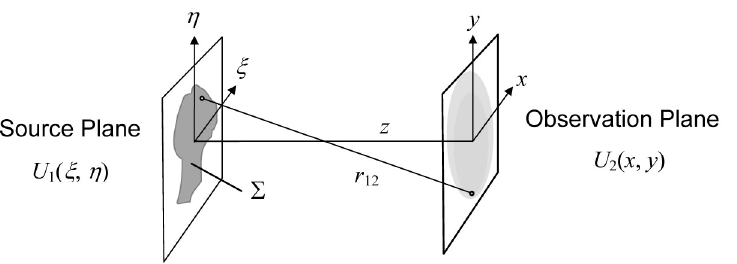
\includegraphics[width = \linewidth]{pics/fresnel-1}
\caption{Source Plane and Observation Plane}
\label{fig:fresnel_1}
\end{figure}
The diffraction effects lie in the Fresnel region since the Fresnel number would be less than one. In this case, the diffraction effects can be given by the equation \ref{eq:fresnel-1}.

\begin{equation}
\label{eq:fresnel-1}
U_2(x,y) = \frac{e^{jkz}}{j\lambda z}\int \int U_1(\xi, \eta )exp(\frac{jk}{2z}[(x - \xi)^2 + (y - \eta)^2])d\xi d\eta
\end{equation}
This expression can also be written in the form of equation \ref{eq:fresnel-2}.
\begin{equation}
\label{eq:fresnel-2}
U_2(x,y) = F^{-1}(F(U_1(x,y)F(h(x,y)))
\end{equation}
where
\begin{equation}
\label{eq:fresnel-3}
h(x,y) = \frac{e^{jkz}}{j\lambda z}exp(\frac{jk}{2z}(x^2 + y^2))
\end{equation}

\section*{Appendix A Camera Dimensions}
This section shows the dimension of the camera module as provided by the camera vendor.

\begin{figure}[!htbp]
\centering
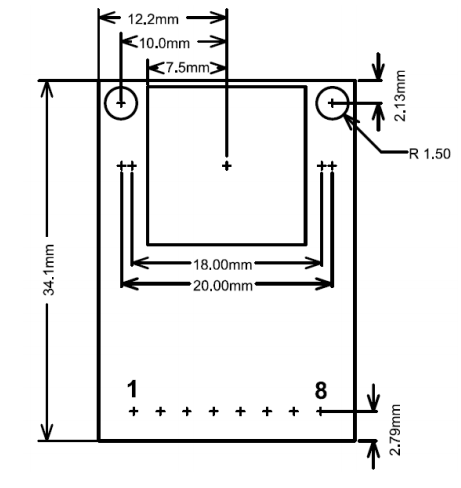
\includegraphics[width = 0.75 \linewidth]{pics/arducam_mech}
\caption{Dimensions of both OV5642 and OV2640 camera modules}
\label{fig:arducam_mech}
\end{figure}

